   
        
        \begin{ledgroupsized}[r]{120mm}
        \footnotesize 
        \pstart        
        \noindent\textbf{\"{U}berlieferung:}  
        \pend
        \end{ledgroupsized}
      
       
              \begin{ledgroupsized}[r]{114mm}
              \footnotesize 
              \pstart \parindent -6mm
              \makebox[6mm][l]{\textit{L}}Konzept: LH XXXV 15, 6 Bl. 64\textendash 65. 1 Bog. 2\textsuperscript{o}. 4 S. zweispaltig. Linke Spalte fortlaufender Text, rechte Spalte umfangreiche Korrekturen und Erg\"{a}nzungen, die auf Bl. 64 r\textsuperscript{o} die rechte Spalte vollst\"{a}ndig ausf\"{u}llen. Auf Bl. 64 v\textsuperscript{o} rechts oben die Zeichnung [Fig. 1]. Die \"{u}brigen Zeichnungen in der oberen H\"{a}lfte der rechten Spalte von Bl. 65 v\textsuperscript{o}. Darunter drei Nebenrechnungen, die nicht zum Text geh\"{o}ren.\\Cc 2, Nr. 484 A \pend
              \end{ledgroupsized}
        \vspace*{8mm}
        \pstart 
        \normalsize
      [64 r\textsuperscript{o}] Ex quo \edtext{horologium funependulo animatum omnibus hactenus cognitis accuratius,  detectum est in}{\lemma{quo}\Afootnote{ \textit{ (1) }\ Illustris Hugenius\protect\index{Namensregister}{\textso{Huygens} (Hugenius, Vgenius, Hugens, Huguens), Christiaan 1629\textendash 1695|textit} horologium\protect\index{Sachverzeichnis}{horologium|textit} omnibus hactenus cognitis accuratius, funependulo\protect\index{Sachverzeichnis}{funependulum|textit} animatum, detexit, in \textit{ (2) }\ horologium [...] in \textit{ L}}} magnam omnes spem erecti sumus. Negotii Longitudinum\protect\index{Sachverzeichnis}{longitudo} aliquando penitus conficiendi \edtext{quantum ab observatione coeli sperari potest}{\lemma{}\Afootnote{quantum [...] potest \textit{ erg.} \textit{ L}}}.
      \edlabel{horologistart} \edtext{Horologio jam accurato}{\lemma{}\xxref{horologistart}{horologiend}\Afootnote{\textit{ (1) }\ Eo \textit{ (2) }\ Tali horologio\protect\index{Sachverzeichnis}{horologium|textit} \textit{ (3) }\ Horologio jam accurato supposito variae \textit{ (a) }\ adhibitae \textit{ (b) }\ propositae sunt \textit{ (aa) }\ coeli \textit{ (bb) }\ loci navis [...] mihi \textbar\ novissime \textit{ gestr.}\ \textbar\ in [...] transigitur, \textit{ (aaa) }\ et \textit{ (bbb) }\ cum contra [...] sed \textit{ (aaaa) }\ non nisi soli simplici \textit{ (bbbb) }\ solo solis \textit{ (aaaaa) }\ Lunaeque\protect\index{Sachverzeichnis}{luna|textit} \textit{ (bbbbb) }\ Lunaeve [...] conspectu \textit{ (aaaaa-a) }\ indiget \textit{ (bbbbb-b) }\ contenta est \textbar\ qui raro per \textit{erg.}\ \textbar\ \textit{ (aaaaa-aa) }\ longum \textit{ (bbbbb-bb) }\ tempus  \textbar\ notabile \textbar\ deesse potest \textit{ erg.} \textbar\ \textit{ erg.} \textbar\ . Cum [...] quae \textit{ (aaaaa-aaa) }\ in Sole\protect\index{Sachverzeichnis}{sol|textit} \textit{ (bbbbb-bbb) }\ \textso{Sole} [...] hoc \textbar\ praeter caetera \textit{ erg.} \textbar\ incommodum [...] facta \textit{ (aaaaa-aaaa) }\ secunda \textit{ (bbbbb-bbbb) }\ posterior aeris \textit{ (aaaaa-aaaaa) }\ navisque \textit{ (bbbbb-bbbbb) }\ marisve [...] Hugenio \textbar\ Horologii penduli\protect\index{Sachverzeichnis}{horologium!pendulum} \textit{ erg.} \textbar\ inventare [...] denique \textbar\ satis \textit{ erg.} \textbar\ est [...] aut facillimo \textit{ (aaaaa-aaaaa-a) }\ indiget, nec \textit{ (bbbbb-bbbbb-b) }\ ac [...] quia \textit{ (aaaaa-aaaaa-aa) }\ a refractionibus\protect\index{Sachverzeichnis}{refractio|textit} \textit{ (bbbbb-bbbbb-bb) }\ sola sideris \textit{ (aaaaa-aaaaa-aaa) }\ conspecti \textit{ (bbbbb-bbbbb-bbb) }\ cujusdam elevatione [...] bonis \textbar\ ad quartas usque minutorum partes  \textbar\ et ultra \textit{ erg.}\ \textbar\ divisis, \textit{ erg.} \textbar\ \textit{erg.} \textbar\ satis \textit{ (aaaaa-aaaaa-aaaa) }\ bene \textit{ (bbbbb-bbbbb-bbbb) }\ recte [...] horizontem. \textit{ (aaaaa-aaaaa-aaaaa) }\ Qui instrumento \textit{ (bbbbb-bbbbb-bbbbb) }\ Nec \textbar\ a \textit{ erg.} \textbar\ refractionibus [...] Astronomis \textit{ (aaaaa-aaaaa-aaaaa-a) }\ computata est \textit{ (bbbbb-bbbbb-bbbbb-b) }\ condita est; [...] assurget. \textit{ erg.} \textit{ L}}} supposito variae propositae sunt loci navis per observationes coelestes inveniendi rationes, alia alia commodior; ex quibus una mihi in mentem venit, universalis admodum et simplex, et satis, ut credo, accurata. \textso{Simplex} quia non nisi una observatione coelesti transigitur, cum contra ubi duabus pluribusque observationibus diverso tempore factis opus est, interea navi\protect\index{Sachverzeichnis}{navis} provecta, difficillima reddatur computatio. \textso{Universalis,} quia nulli fere tempori, non diei, non nocti, non certis siderum altitudinibus\protect\index{Sachverzeichnis}{altitudo sideris} alligata est; sed solo solis\protect\index{Sachverzeichnis}{sol} Lunaeve aut stellae cujusdam fixae\protect\index{Sachverzeichnis}{stella!fixa} conspectu contenta est
 %\edtext{qui raro per tempus notabile deesse potest}{\lemma{} \Afootnote{qui raro per \textit{ (1) }\ longum \textit{ (2) }\ tempus  \textbar\ notabile \textbar\ deesse potest \textit{ erg.} \textbar\ \textit{ erg.} \textbar\ \textit{ L}}}. Cum contra solutiones quae ex \textso{Lunae}\protect\index{Sachverzeichnis}{luna} observatione pendent, dimidio fere mensis tempore ante et post novilunium conspectu scilicet Lunae\protect\index{Sachverzeichnis}{luna} negato, cessent, et quae \edtext{\textso{Sole}}{\lemma{quae}\Afootnote{ \textit{ (1) }\ in Sole\protect\index{Sachverzeichnis}{sol|textit} \textit{ (2) }\ \textso{Sole} \textit{ L}}} indigent, noctu fieri nequeant; et eae in quibus duabus aequalibus ejusdem sideris altitudinibus\protect\index{Sachverzeichnis}{altitudo sideris} observatis opus est, hoc \edtext{praeter caetera}{\lemma{}\Afootnote{praeter caetera \textit{ erg.} \textit{ L}}} incommodum habeant, ut priore observatione facta \edtext{posterior}{\lemma{facta}\Afootnote{ \textit{ (1) }\ secunda \textit{ (2) }\ posterior \textit{ L}}} aeris \edtext{marisve}{\lemma{aeris}\Afootnote{ \textit{ (1) }\ navisque \textit{ (2) }\ marisve \textit{ L}}} injuria facile intercipiatur, ac proinde prior reddatur inutilis. De quibus aliisque in hoc negotio observandis legi possunt, tum quae ab Illustri Hugenio\protect\index{Namensregister}{\textso{Huygens,} Christiaan (1629\textendash 1695)} \edtext{Horologii penduli\protect\index{Sachverzeichnis}{horologium!pendulum}}{\lemma{}\Afootnote{Horologii penduli\protect\index{Sachverzeichnis}{horologium!pendulum} \textit{ erg.} \textit{ L}}} inventore circa applicationem ejus ad Longitudines\protect\index{Sachverzeichnis}{longitudo} sunt scripta, \edtext{}{\lemma{scripta,}\Bfootnote{\textsc{Chr. Huygens, }\cite{00063}\textit{Br\`{e}ve instruction}, Paris 1665 (\textit{HO} V, S.~214\textendash 230).}} tum quae Transactionibus Anglicanis num. 47. sunt inserta.\edtext{}{\lemma{inserta.}\Bfootnote{\textsc{Chr. Huygens, }\cite{00064}\textit{Instructions concerning the use of pendulum\textendash watches}, \textit{Philosophical Transactions}, Bd 4, Nr. 47, 1669, S.~937\textendash 953 (\textit{HO} VI, S.~446\textendash 459). }} \textso{Accurata} denique \edtext{satis}{\lemma{}\Afootnote{satis \textit{ erg.} \textit{ L}}} est quam propono, ratio, tum quia calculo exiguo aut facillimo \edtext{ ac ne nautas quidem turbaturo indiget}{\lemma{facillimo}\Afootnote{ \textit{ (1) }\ indiget, nec \textit{ (2) }\ ac [...] indiget \textit{ L}}} tum quia \edtext{sola}{\lemma{quia}\Afootnote{ \textit{ (1) }\ a refractionibus\protect\index{Sachverzeichnis}{refractio|textit} \textit{ (2) }\ sola \textit{ L}}} sideris\protect\index{Sachverzeichnis}{sidus} 
 qui raro per tempus notabile deesse potest. Cum contra solutiones quae ex \textso{Lunae}\protect\index{Sachverzeichnis}{luna} observatione pendent, dimidio fere mensis tempore ante et post novilunium conspectu scilicet Lunae\protect\index{Sachverzeichnis}{luna} negato, cessent, et quae \textso{Sole }indigent, noctu fieri nequeant; et eae in quibus duabus aequalibus ejusdem sideris altitudinibus\protect\index{Sachverzeichnis}{altitudo sideris} observatis opus est, hoc praeter caetera incommodum habeant, ut priore observatione facta posterior aeris marisve injuria facile intercipiatur, ac proinde prior reddatur inutilis. De quibus aliisque in hoc negotio observandis legi possunt, tum quae ab Illustri Hugenio\protect\index{Namensregister}{\textso{Huygens} (Hugenius, Vgenius, Hugens, Huguens), Christiaan 1629\textendash 1695} Horologii penduli\protect\index{Sachverzeichnis}{horologium!pendulum} inventore circa applicationem ejus ad Longitudines\protect\index{Sachverzeichnis}{longitudo} sunt scripta, \edtext{}{\lemma{scripta,}\Bfootnote{\textsc{Chr. Huygens}, \cite{00212}\textit{Kort onderwijs}, Den Haag 1665 (\textit{HO} XVII, S.~199\textendash 237).}} tum quae Transactionibus Anglicanis num. 47. sunt inserta.\edtext{}{\lemma{inserta.}\Bfootnote{\textsc{Chr. Huygens, }\cite{00064}\textit{Instructions concerning the use of pendulum-watches}, \textit{PT} 4 (1669), S.~937\textendash 953 (\textit{HO} VI, S.~446\textendash 459). }} \textso{Accurata} denique satis est quam propono, ratio, tum quia calculo exiguo aut facillimo ac ne nautas quidem turbaturo indiget tum quia sola sideris\protect\index{Sachverzeichnis}{sidus} cujusdam elevatione ultra Horizontem loci navis\protect\index{Sachverzeichnis}{navis} observata, quae certe instrumentis bonis ad quartas usque minutorum partes et ultra divisis, satis recte sumi potest, perficitur: neque enim nisi angulo indigemus, quem radius e sidere\protect\index{Sachverzeichnis}{sidus} dato ductus facit ad loci horizontem. Nec a refractionibus\protect\index{Sachverzeichnis}{refractio} metuere nobis magnopere debemus praeterquam enim quod sideris\protect\index{Sachverzeichnis}{sidus} ultra horizontem satis evecti refractio\protect\index{Sachverzeichnis}{refractio} minus turbat, et Tabula etiam computandarum Refractionum\protect\index{Sachverzeichnis}{refractio} ex crepusculorum quantitate aliisque indiciis ab Astronomis condita est; praeter inquam haec omnia en facilem occurrendi rationem. Si eodem tempore duo pluraque sidera\protect\index{Sachverzeichnis}{sidus} (semper enim plures fixae\protect\index{Sachverzeichnis}{stella!fixa} simul videntur) observentur, cum enim eorum refractionem\protect\index{Sachverzeichnis}{refractio} necesse sit esse diversam, sese mutuo corrigent observationes, quae cum eodem tempore fiant, uni observationi aequipollent. Utile autem est sidus\protect\index{Sachverzeichnis}{sidus} eligi, prae caeteris quod alte supra horizontem loci assurget.\edlabel{horologiend}      
 \pend \pstart \edtext{Constat locum navis praecise cognosci cognita Latitudine longitudineque loci, et longitudinem cognosci cognita}{\lemma{Constat}\Afootnote{ \textit{ (1) }\ ad locum navis\protect\index{Sachverzeichnis}{navis|textit} cognitionem necessariam esse \textit{ (2) }\ ad locum navis\protect\index{Sachverzeichnis}{navis|textit} cognoscendum necessariam esse cognitionem Latitudinis\protect\index{Sachverzeichnis}{latitudo|textit} longitudinisque\protect\index{Sachverzeichnis}{longitudo|textit} loci, et ad cognitionem longitudinis\protect\index{Sachverzeichnis}{longitudo|textit} \textit{ (3) }\ locum [...] cognita \textit{ L}}} hora praesenti tum loci navis\protect\index{Sachverzeichnis}{navis} per observationem coeli, tum loci discessus per observationem \edtext{horologii}{\lemma{observationem}\Afootnote{ \textit{ (1) }\ penduli\protect\index{Sachverzeichnis}{pendulum|textit} \textit{ (2) }\ horologii \textit{ L}}} accurati inde a loco discessus in navi\protect\index{Sachverzeichnis}{navis} \edlabel{allatistart}allati.\pend \pstart \edtext{Seposito horologio seu hora presenti loci\edlabel{allatiend}}{\lemma{allati.}\xxref{allatistart}{allatiend}\Afootnote{ \textit{ (1) }\ Horam loci \textit{ (2) }\ Seposito horologio seu hora  \textbar\ presenti \textit{ erg.}\ \textbar\ loci \textit{ L}}} discessus, tantum de hora navis\protect\index{Sachverzeichnis}{navis} seu coeli observatione hoc loco dicam. Ad Horam loci computandam, sufficere cognitionem \textso{Latitudinis}\protect\index{Sachverzeichnis}{latitudo} loci, et declinationis solaris\protect\index{Sachverzeichnis}{declinatio!solaris}, vulgo constat. Hugenius\protect\index{Namensregister}{\textso{Huygens} (Hugenius, Vgenius, Hugens, Huguens), Christiaan 1629\textendash 1695}\edtext{}{\lemma{Hugenius}\Bfootnote{\textsc{Chr. Huygens}, \cite{00212}\textit{Kort onderwijs}, Den Haag 1665, S. 20\textendash 28 (\textit{HO} XVII, S. 218\textendash 226).}} rationem proposuit \edtext{quae}{\lemma{proposuit}\Afootnote{ \textit{ (1) }\ commodiorem, quae neque \textit{ (2) }\ quae \textit{ L}}} neutra indigeret\edtext{ observatis tantum duabus}{\lemma{indigeret}\Afootnote{ \textit{ (1) }\ sed fieret factis duabus observationibus \textit{ (2) }\ observatis  \textbar\ tantum \textit{ erg.}\ \textbar\ duabus \ \textit{ L}}} aequalibus solis\protect\index{Sachverzeichnis}{sol} aut etiam alterius stellae\protect\index{Sachverzeichnis}{stella} \edtext{satis alte super horizontem emergentis }{\lemma{}\Afootnote{satis alte super horizontem emergentis  \textbar\ (quanquam hoc cognosci non possit, \textit{ (1) }\ nisi qua \textit{ (2) }\ altene an non assurrectura sit, nisi altitudine loci circiter cognita) \textit{ gestr.}\ \textbar\  \textit{ erg.} \textit{ L}}}\edtext{altitudinibus}{\lemma{emergentis}\Afootnote{ \textit{ (1) }\ observationibus \textit{ (2) }\ altitudinibus \textit{ L}}} \edtext{aut unica sed tunc facta, cum sidus\protect\index{Sachverzeichnis}{sidus} est praecise in meridiano\protect\index{Sachverzeichnis}{meridianus} loci.}{\lemma{}\Afootnote{aut [...] loci. \textit{ erg.} \textit{ L}}} \edtext{ Optimum esse eligere altitudines}{\lemma{loci.}\Afootnote{ \textit{ (1) }\ Ex quibus  \textbar\ duabus \textit{ erg.}\ \textbar\ altitudinib \textit{ (2) }\ Optimum \textit{(a)}\ est autem \textit{(b)}\ esse eligere altitudines \textit{ L}}} minimas, id est ipsum praecise tempus solis\protect\index{Sachverzeichnis}{sol} surgentis aut cadentis \edtext{observato momento quo dimidia solis\protect\index{Sachverzeichnis}{sol} pars extat supra horizontem, dimidia infra horizontem deprimitur.}{\lemma{}\Afootnote{observato \textit{ (1) }\ tempo \textit{ (2) }\ momento \textbar\ quo [...] deprimitur. \textit{ erg.} \textbar\ \textit{ L}}} \edtext{Nave autem interea progrediente differentiam locorum cujusque observationis}{\lemma{deprimitur.}\Afootnote{ \textit{ (1) }\ Tempus autem inter utramque observationem elapsum eorum \textit{ (2) }\ Nave [...] observationis \textit{ L}}} illa ipsa ratione, qua vulgo nautae in mensuranda per conjecturas navis\protect\index{Sachverzeichnis}{navis} via utuntur, definiendam.\pend\pstart Caeterum quod \edtext{ad hunc calculum}{\lemma{quod}\Afootnote{ \textit{ (1) }\ hac ratione observat \textit{ (2) }\ ad hunc calculum \textit{ L}}} \edtext{Longitudinum cognitio Latitudinum}{\lemma{calculum}\Afootnote{ \textit{ (1) }\ \textso{Latitudinis}\protect\index{Sachverzeichnis}{latitudo|textit} \textit{ (2) }\ Longitudinum cognitio Latitudinum \textit{ L}}} necessaria non est, id quidem mea sententia lucro caret, indaganda enim nihilominus Latitudo\protect\index{Sachverzeichnis}{latitudo} est separatim, ut locus navis\protect\index{Sachverzeichnis}{navis} verus inveniatur, nam uti \edtext{Latitudo}{\lemma{uti}\Afootnote{ \textit{ (1) }\ Longitudo\protect\index{Sachverzeichnis}{longitudo|textit} \textit{ (2) }\ Latitudo \textit{ L}}} sine Longitudine\protect\index{Sachverzeichnis}{longitudo}, ita \edtext{vicissim longitudo}{\lemma{ita}\Afootnote{ \textit{ (1) }\ longitudine\protect\index{Sachverzeichnis}{longitudo|textit} \textit{ (2) }\ vicissim longitudo \textit{ L}}} sine latitudine\protect\index{Sachverzeichnis}{latitudo} ad regendam navigationem non sufficit.\pend \pstart Accedit, quod magna spes est \textso{Rationem }\textso{Latitudinum}\protect\index{Sachverzeichnis}{latitudo}\textso{ investigandarum universalem} ab observatione coeli et tempestatibus independentem quamprimum plene detectum iri, ubi modo \textso{Acus inclinatoria}\protect\index{Sachverzeichnis}{acus!inclinatoria} ad regulam reducta fuerit, quod mihi jam in potestate nostra esse videtur \edtext{ut postea fusius dicam.}{\lemma{}\Afootnote{ut postea fusius dicam. \textit{ erg.} \textit{ L}}}\footnote{\textit{In der rechten Spalte}: Verte et vide sign. \female. Sequuntur enim verba: Quod ergo hoc modo.} Constat enim acum \edtext{puram}{\lemma{acum}\Afootnote{ \textit{ (1) }\ magneticam \textit{ (2) }\ puram \textit{ L}}}, ubi primum magneti\protect\index{Sachverzeichnis}{magnes} affricta est, \edtext{quasi pondusculo appenso in nostris}{\lemma{est,}\Afootnote{ \textit{ (1) }\ in nostri quasi pondere \textit{ (2) }\ quasi pondusculo appenso in nostris \textit{ L}}} oris nonnihil versus polum arcticum\protect\index{Sachverzeichnis}{polus!arcticus} propendere; et \edtext{quanto}{\lemma{}\Afootnote{quanto \textbar\ illuc \textit{ gestr.}\ \textbar\ propius \textit{ L}}} propius accedat polo\protect\index{Sachverzeichnis}{polus}, eo \edtext{magis inclinari}{\lemma{eo}\Afootnote{ \textit{ (1) }\ fieri \textit{ (2) }\ magis inlinari \textit{ L}}}; donec in Regionibus Arcticis \edtext{ad situm}{\lemma{}\Afootnote{ad situm \textit{ erg.} \textit{ L}\ \hspace{10mm}5\hspace{3mm} ergo \textbar\ Illustris Hugenius\protect\index{Namensregister}{\textso{Huygens} (Hugenius, Vgenius, Hugens, Huguens), Christiaan 1629\textendash 1695} \textit{ gestr.}\ \textbar\ hoc \textit{ L}}} perpendicularem propemodum accedat.\pend 
    %Figur aus 64v aus satztechnischen Gruenden hier eingefuegt
    \vspace{0.5ex}
    \begin{center}          
    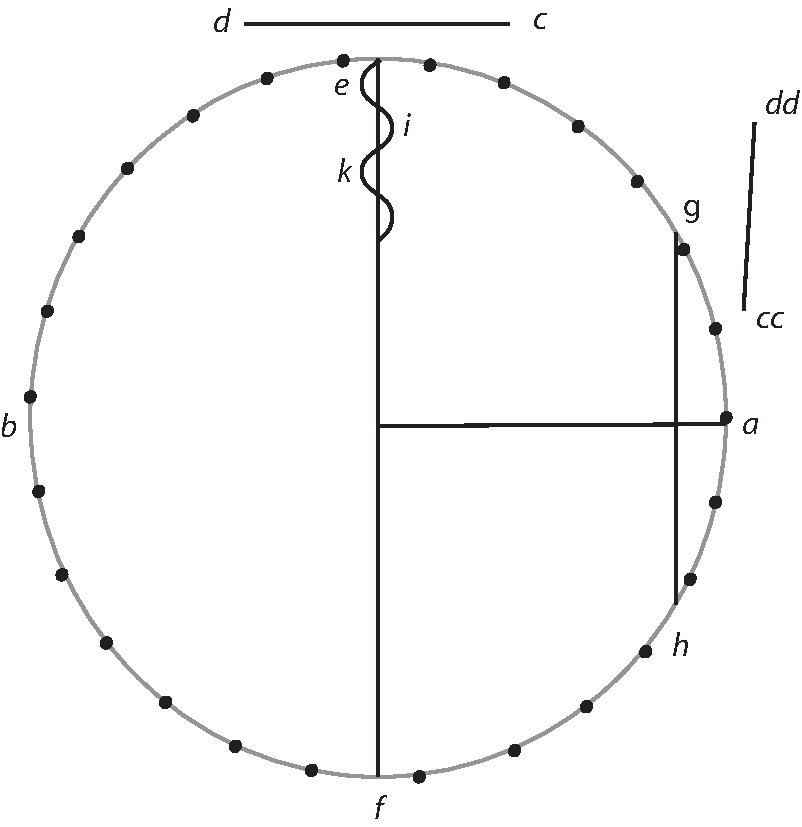
\includegraphics[width=0.65\textwidth]{images/35_15_6_64v}
    \\\textit{[Fig. 1, tlw. Blindzeichnung]}
    \end{center}
 \pstart Quod nautae illuc euntes malo suo experti sunt. Unde illi contraria \edtext{seu ant\-arcticum polum\protect\index{Sachverzeichnis}{polus!antarcticus} respiciente}{\lemma{}\Afootnote{seu ant\-arcticum polum\protect\index{Sachverzeichnis}{polus!antarcticus} respiciente \textit{ erg.} \textit{ L}}} acus\protect\index{Sachverzeichnis}{acus!magnetica} parte magis cis lineam gravata, aut trans lineam levata; acum in aequilibrium\protect\index{Sachverzeichnis}{aequilibrium} redigere conantur. Hujus rei